% vim: set textwidth=78 autoindent:

\subsection{Complemento GPS}\label{label_plugingps}

% when the revision of a section has been finalized, 
% comment out the following line:
% \updatedisclaimer

\subsubsection{¿ Qué es GPS?}\label{whatsgps}

GPS, el Sistema Global de Posicionamiento, es un sistema basado en satélite que permite a cualquiera con un receptor GPS encontrar su posición exacta en cualquier lugar en el mundo.
Es usado como auxiliar en la navegación, por ejemplo en aeroplanos, en botes y por excursionistas.
El receptor GPS usa las señales de satélites para calcular su latitud, longitud, y (algunas veces) elevación.
La mayoría de los receptores tienen la capacidad de almacenar lugares (conocidos como \emph{waypoints}), secuencias de lugares que forman una \emph{ruta} planeada y un tracklog o \emph{track} de los movimientos de los receptores en el tiempo.
Waypoints, rutas y tracks solo los tres tipos de objetos básicos en datos GPS.
QGIS muestra waypoints en capas de puntos mientras que las rutas y tracks son mostrados en capas de cadena de líneas.

\subsubsection{Cargar datos GPS desde un archivo}\label{label_loadgps}

Hay docenas de diferentes formatos de archivo para almacenar datos GPS.
El formato que QGIS usa es llamado GPX (GPS eXchange format), el cual es un formato de intercambio estandar que puede contener cualquier número de waypoints, rutas y tracks en el mismo archivo.

Para cargar una archivo GPX  primero necesita cargar el complemento.
\mainmenuopt{Complementos} > \dropmenuopttwo{mActionShowPluginManager}{Administrador de complementos...} > \checkbox{Herramientas GPS}. Cuando este complemento es cargado un botón con un pequeño dispositivo GPS de mano será mostrado en la barra de herramientas. Un ejemplo de archivo GPX está disponible en el conjunto de datos de ejemplo de QGIS:
\filename{/qgis\_sample\_data/gps/national\_monuments.gpx}. Vea 
la sección~\ref{label_sampledata} para mas información acerca de los datos de ejemplo.

\begin{enumerate}
\item Clic en el ícono \toolbtntwo{gps_importer}{Herramientas GPS} y abra la
pestaña \tab{Cargar archivo GPX} (vea la figura \ref{figure gpxloader}).
\item \button{Explorar} al directorio \filename{qgis\_sample\_data/gps/},
seleccione el archivo GPX \filename{national\_monuments.gpx} y haga clic \button{Abrir}.
\end{enumerate}

\begin{figure}[ht]
   \begin{center}
\caption{\label{gpxloader}El diálogo de \emph{Herramientas GPS} \nixcaption}
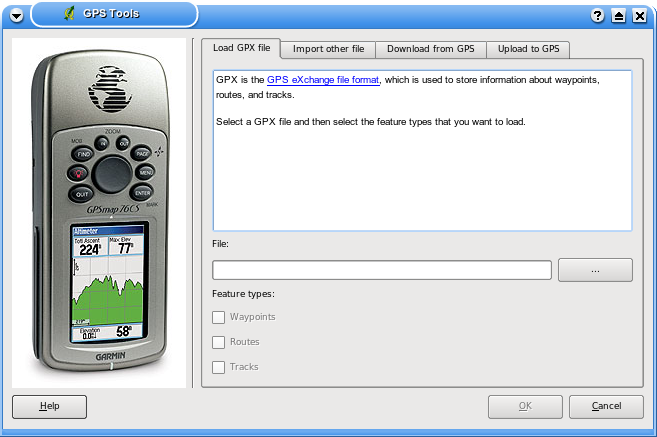
\includegraphics[clip=true, width=12cm]{loadgpx}
\end{center}
\end{figure}

Use el botó explorar \browsebutton para seleccionar el archivo GPX, entonces use las
cajas de verificación para seleccionar los tipos de objetos espaciales que desea cargar desde el archvo GPX.
Cada tipo de objeto espacial será cargado en una capa separada cuando haga clic en \button{OK}.
El archivo \filename{national\_monuments.gpx} solo incluye waypoints.

\subsubsection{GPSBabel}

Dado que QGIS usa archivos GPX necesita una forma de convertir otros formatos de archivo GPS a GPX.
Esto puede ser realizado para muchos formatos usando el programa gratuito GPSBabel, el cual está disponible en \url{http://www.gpsbabel.org}.
Este programa también puede transferir datos GPS entre su computadora y un dispositivo GPS.
QGIS usa GPSBabel para hacer esas cosas, de manera que es recomendable que lo instale.
Sin embargo, si solo desea cargar datos GPS desde archivos GPX no lo necesitará.
La versión 1.2.3 de GPSBabel trabaja con QGIS, pero usted podrá usar cualquier versión posterior sin problemas.


\subsubsection{Importar datos GPS}

Para importar datos GPS desde un archivo que no es un archivo GPX, use la herramienta \tab{Importar otro archivo} en el diálogo de Herramientas GPS.
Aquí selecciona el archivo que desea importar (y el tipo de archivo), cuales tipos de objeto desea importar de el, donde desea almacenar los archivos GPX convertidos y el nombre de la nueva capa. Note que no todos los formatos de datos GPS soportarán los tres tipos de objetos, de manera que para muchos formatos solo podrá elegir entre uno o dos tipos.  


\subsubsection{Descargar datos GPS desde un dispositivo}

QGIS puede usar GPSBabel para descargar datos desde un dispositivo GPS directamente como una nueva capa vectorial.
Para esto usamos la pestaña \tab{Descargar desde GPS} del diálogo de Herramientas GPS(vea la figura \ref{figure_download}). Aquí, seleccionamos el tipo de dispositivo GPS, el puerto al que está conectado (o usb si su GPS lo suporta), el tipo de objeto que quiere bajar, el archivo GPX donde los datos deberían ser almacenados, y el nombre de la nueva capa.

\begin{figure}[ht]
   \begin{center}
\caption{\label{figure_download}La herramienta para descargar \nixcaption}
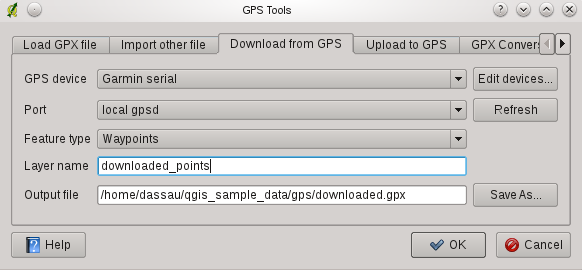
\includegraphics[clip=true, width=12cm]{download}
   \end{center}
\end{figure}

El tipo de dispositivo que seleccione en el menú de dispositivo GPS determina como GPSBabel trata de comunicarse con su dispositivo GPS.
Si ninguno de los tipos disponibles trabajan con su dispositivo GPS puede crear un nuevo tipo (vea la sección \ref{sec:Defining-new-device}).

El puerto puede ser un nombre de archivo o algún otro nombre que su sistema operativo use como referencia al puerto físico en su computadora a la que el dispositivo GPS está conectado. Puede ser simplemente usb, para unidades GPS usb.
\nix en Linux esto es algo como esto /dev/ttyS0 o /dev/ttyS1 y en \win Windows es COM1 o COM2.

Cuando hace clic \button{OK} los datos serán descargados del dispositivo y aparecen como una capa en QGIS.

\subsubsection{Cargar datos GPS a un dispositivo}

También puede cargar datos directamente de una capa vectorial en QGIS a un dispositivo GPS usando la pestaña \tab{Cargar a GPS} del diálogo herramientas GPS. Para hacer esto simplemente seleccione la capa que desea cargar (la cual debe ser una capa GPX), 
su tipo de dispositivo GPS, y el puerto(o usb) al cual está conectado.
Al igual que la herramienta de descarga puede especificar nuevos tipos de dispositivos si su dispositivo no está en la lista.

Esta herramienta es muy útil en combinación con las capacidades de edición de vectores de QGIS. Te permite cargar un mapa, crear waypoints y rutas, y después cargarlas y usarlas en su dispositivo GPS.

\subsubsection{\label{sec:Defining-new-device}Definir nuevos tipos de dispositivos}

Hay muchos diferentes tipos de dispositivos GPS.
Los desarrolladores de QGIS no pueden probar a todos ellos, de manera que si usted tiene uno que no trabaja con alguno de los dispositivos listados en la pestañas de herramientas \tab{Descargar de GPS} y \tab{Cargar a GPS} puede definir su propio dispositivo.
Usted hace esto usando el editor de dispositivos GPS, el cual inicia haciendo clic en el botón \button{Editar dispositivos} en las pestañas de descarga y carga.

Para definir un nuevo dispositivo simplemente haga clic en el botón \button{Nuevo dispositivo}, capture un nombre, un comando para descarga y un comando para descarga para su dispositivo, y clic en el botón \button{Actualizar dispositivo}.
El nombre será listado en los menús de dispositivos en las ventanas de carga y descarga, y puede ser cualquier cadena.
El comando de descarga es el comando que es usado para descargar datos del dispositivo a un archivo GPX.
Este será probablemente un comando de GPSBabel, pero puede usar cualquier otro programa de línea de comandos que pueda crear un archivo GPX.
QGIS reemplazará las palabras clave \usertext{\%type}, \usertext{\%in}, and \usertext{\%out} cuando ejecute el comando.

\usertext{\%type} será reemplazado por {}``\usertext{-w}'' si está descargando waypoints, {}``\usertext{-r}'' si está descargando rutas y {}``\usertext{-t}'' si está descargando tracks.
Estas son opciones de línea de comandos que dicen a GPSBabel cual tipo de objeto espacial descargar.

\usertext{\%in} será reemplazado por el nombre del puerto que eligió en la ventana de descarga y \usertext{\%out} será reemplazado por el nombre que eligió para el archivo GPX donde los datos serán almacenados.
De manera que si crea un tipo de dispositivo con el comando de descarga {}``\usertext{gpsbabel \%type -i garmin -o gpx \%in \%out}'' (este es actualmente el comando de descarga para el tipo de dispositivo predefinido \selectstring{Dispositivo GPS:}{Garmin serial})y entonces úselo para descargar waypoints del puerto {}``\usertext{/dev/ttyS0}'' al archivo {}``\usertext{output.gpx}'', QGIS reemplazará las palabras clave y ejecutar el comando {}``\usertext{gpsbabel -w -i garmin -o gpx /dev/ttyS0 output.gpx}''.

El comando de carga es el comando que es usado para cargar datos a los dispositivos.
Las mismas palabras clave son usadas, pero, \usertext{\%in} es ahora reemplazado por el nombre  del archivo GPX  para la capa que está siendo cargada, y \usertext{\%out} es reemplazado por el nombre del puerto.

Puede aprender mas acerca de GPSBabel y la lista de comandos disponibles en \url{http://www.gpsbabel.org}

Una vez que ha creado un nuevo tipo de dispositivo este aparecerá en la lista de dispositivos para las herramientas de carga y descarga.
